% Objective of the quantitative analysis
This section presents the quantitative analysis of the model with three main objectives: to reproduce the labor share dynamics observed over the period 1950 to 2010, to provide model predictions after 2010, and to understand the transmission channels of demographic effects on the labor share. I compute model predictions for France and the United States. I focus on these two countries because they face important changes in the age structure of the population due to the emergence of the boomers' generation, while having sizeable differences in terms of labor market institutions and public policy.

% Follow the methodology of Gonzalez-Eiras and Niepelt
To simulate the model, I follow the methodology of \citet{Gonzalez-Eiras2012Ageing} which is standard in the literature to calibrate an OLG model. One period in the model is assumed to correspond to 40 years in the data. Thus, households are considered as young between 20 and 60 years of age and as old thereafter.\footnote{An implicit assumption of the model is that the retirement age is constant. The average French effective retirement age was 67.8 in 1970 and has declined to 59.3 in 2010. In the US it has gone from 68.4 to 65.6 over the same period (data from the \href{https://www.oecd.org/els/emp/average-effective-age-of-retirement.htm}{OECD Database, Ageing and Employment Policies - Statistics on average effective age of retirement}). I suppose, as an approximation, that agents retire at 60 years old to match the period lengths of the calibration. Such an assumption should not affect the voting outcome because almost-retired agents may anticipate their future situation once they vote. Nonetheless, a 5-year change remains moderate compared to the 40 years between two periods.}
I compute four sequences of model predictions with a period length of 40 years each. Periods of the first sequence correspond to 1950, 1990, 2030, 2070; for the second sequence to 1960, 2000, 2040, 2080; for the third sequence to 1970, 2010, 2050, 2090; and for the fourth sequence to 1980, 2020, 2060, 2100. When I report time-series predictions, I list these four sequences in a single time series. Thus, there are always eight generations living simultaneously, four of them being young and the four others old. Every 10 years, a new generation is born and an old one dies.

\subsection{Data}\label{chap1-data}

\textbf{Demography.} I use demographic data from the \href{https://population.un.org/wpp/}{United Nations World Population Prospects 2017}.%
\footnote{Demographic data from 1950 to 2010 come from the \href{https://population.un.org/wpp/}{United Nations World Population Prospects 2017}. For future dynamics, I rely on the ``medium variant'' estimates from the United Nations. Demographic data before 1950 are from \href{http://www.populstat.info}{http://www.populstat.info}. Due to data limitations, the expected survival rate $p_{t+1}$ is not available after 2060. Thus, I suppose that $p_{t+1}$ grows at its observed average growth rate until 2060, for each country, hence, 4.921\% for France and 4.137\% for the United States. Nevertheless, I limit my analysis to 4 periods (hence 2100) due to the large degree of uncertainty thereafter.}
I start by computing the old-age dependency ratio from the data as the number of old individuals divided by the number of young ones. Then, I compute the population growth rate using the ratio between the number of young individuals relative to the number of young people in the previous period of the sequence, i.e. $n_t = N_t^y/N_{t-1}^y$. Lastly, the survival rate verifies the identity and equals the product of the old-age-dependency ratio and the population growth, i.e. $p_t \equiv N_t^o/N_t^y\times n_t$. Figure \ref{chap1-fig:demo} plots demographic dynamics for France and the United States and indicates that both countries face the same demographic context.
\begin{figure}[!tb]
	\centering
	\caption{Demographic dynamics}\label{chap1-fig:demo}
	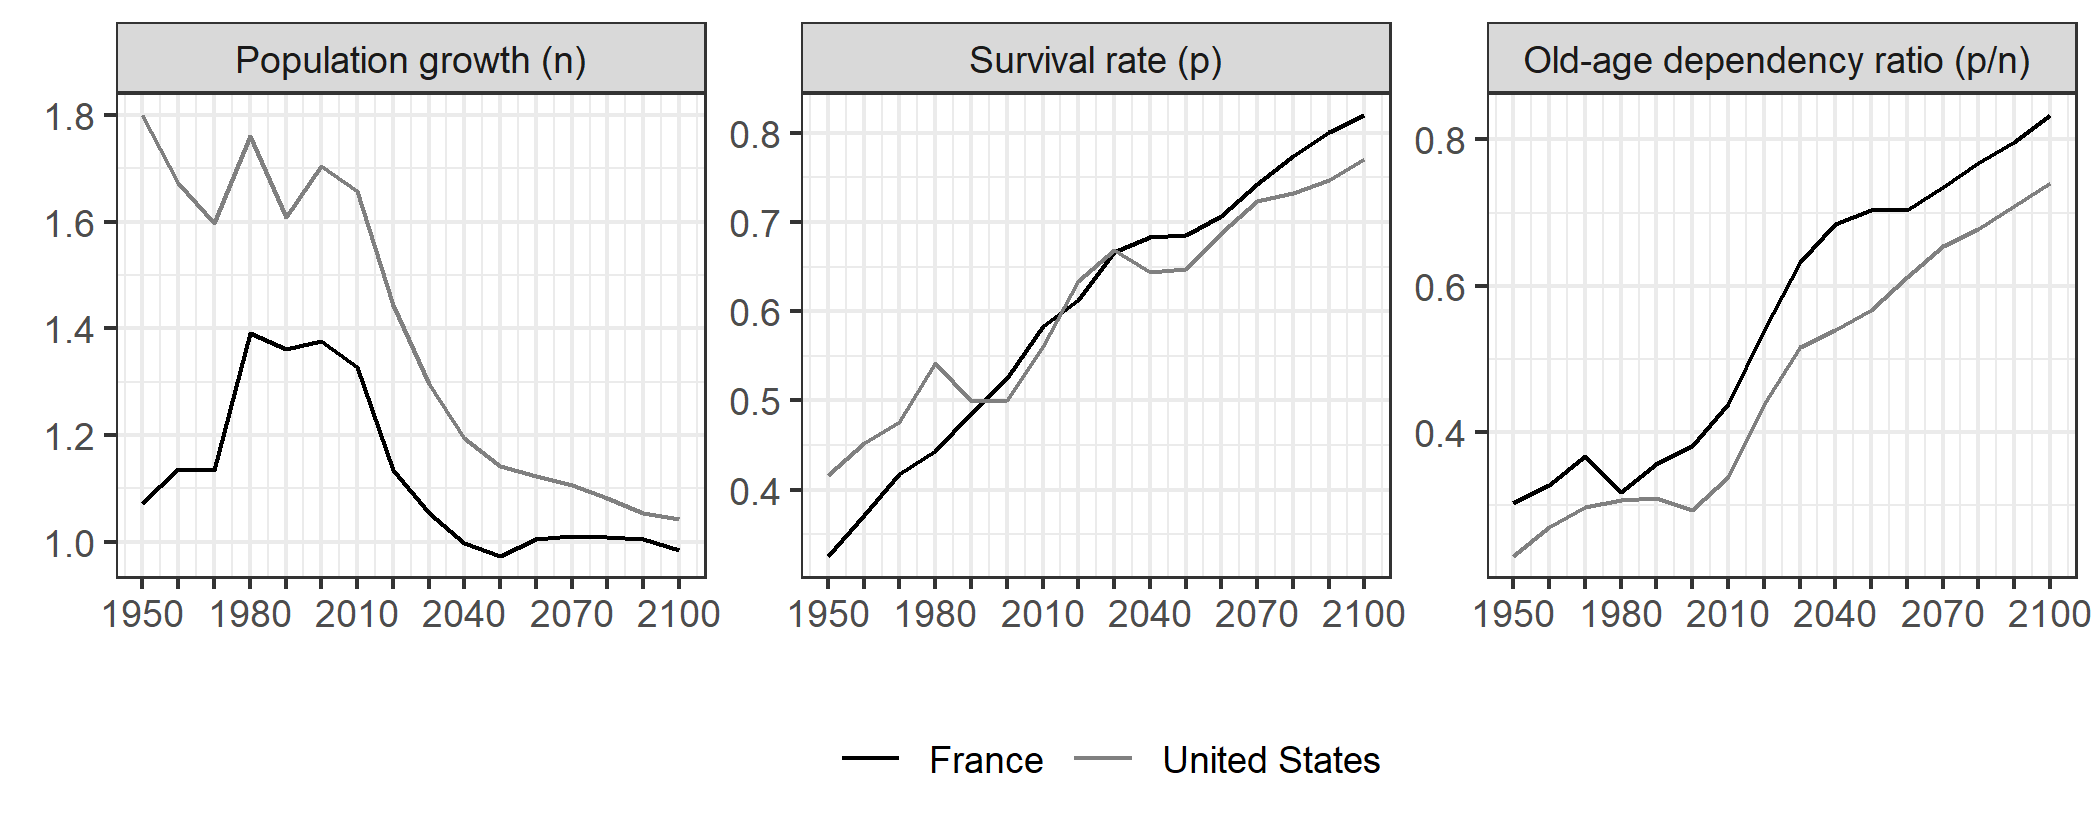
\includegraphics[width=\linewidth]{chap1/graphic/quant-demo.png}
	\vspace{-3em}
	\justify\singlespacing\footnotesize\textit{Notes:} The figure displays, for each country every 10 years, the population growth rate, the survival rate and the old-age dependency ratio. Data correspond to the ``medium variant'' estimates from the  \href{https://population.un.org/wpp/}{United Nations World Population Prospects 2017}.
\end{figure}
I distinguish three eras in terms of dynamics that correspond to the life cycle of the boomers' generation: when the boomers are young between 1970 and 2010; when they retire; and thereafter once they disappeared. Until 2010, the old-age dependency ratio remains roughly stable due to the massive entry of the boomers into the labor force that offsets the rise in the survival rate due to increasing life expectancy. Thereafter, as the boomer generation retires, the survival rate continues to grow and population growth declines. As a consequence, the old-age dependency ratio explodes.

\textbf{Labor share.} I use labor share data from the \href{https://www.rug.nl/ggdc/productivity/pwt/}{Penn World Table 10.0} (PWT); see \citet{Feenstra2015Next} for more details on these data. In this dataset, the labor share $\theta_t$ corresponds to the share of labor compensation in GDP. As argued by \citet{Gollin2002Getting}, the measurement of the labor share is influenced by the adjustment method to take into account self-employed income. In the theoretical framework, workers are young individuals and supply only labor. In line with the model, I consider self-employed income as labor compensation.

\textbf{Capital stock.} I use the capital stock at constant 2011 national prices from the PWT for the capital stock $K_t$. To disentangle the effect of changes in the number of hours worked, I adjust both variables by the average annual hours worked by persons engaged from the same data source.

\textbf{Labor and unemployment.} I also use the number of persons in employment from the PWT. In the model, labor supply is inelastic and there is no distinction between unemployed and inactive individuals. The unemployed, in terms of the model specification, correspond to all agents that do not work. However, in high-income countries such as France and the United States, inactive people also benefit from redistribution through transfer payments. Therefore, I treat them as unemployed and the redistribution is captured through unemployment benefit $b_t$ in the model. I compute the unemployment rate such that $u_t = 1 - emp_t/N^{15-64}_t$, where $emp_t$ is the number of persons in employment and $N_t^{15-64}$ is the working-age population.\footnote{I consider the whole working-age population instead of the young population. Due to the demographic specification of the model, young agents correspond to those between 20 and 60 years old. Data on the number of persons engaged per age group are not available in PWT. Therefore, taking only $N^y_t$ as denominator would bias downward the unemployment rate. % Results are robust to different specifications of the unemployment rate.
Although there are other sources of population data, I rely on the PWT to have consistency using the same data source for input factors and output.}
Then, I compute labor according to the identity $L_t\equiv(1-u_t)N_t^y$.

\textbf{Public policy variables.} I use the government revenue as a share of GDP from the \href{https://www.oecd.org/tax/tax-policy/tax-database/}{OECD Tax Database} to proxy the tax rate $\tau_t$, these data are not available before 1970. I use the pension spending expressed in percentage of GDP as a measure of the old-age specific government spending, i.e. $g_tN^o_t/Y_t$, as it is likely to be positively correlated with. Lastly, I consider the public unemployment spending expressed in percentage of GDP for the share of total unemployment benefits, i.e. $b_tu_tN^y_t/Y_t$. Both latter variables are from the OECD data.

\textbf{Normalization.} 
I normalize the capital-labor ratio $k_t$ and the young population $N_t^y$ to their 1950 values. $L_t$ is computed such that the unemployment rate $u_t$ matches the one derived for 1950 and $K_t$ satisfies the identity $k_t \equiv K_t/L_t$.

\subsection{Calibration}\label{chap1-calibration}

% Calibration
Once stock variables are normalized, I calibrate the parameters of the model $\{ \alpha,$ $\phi,$ $\sigma,$ $\omega,$ $\beta,$ $A \}$. Table \ref{chap1-tab:quant-param} summarizes parameters for both countries.
\begin{table}[!tb]
    \centering
    \begin{threeparttable}
        \caption{Parameters} \label{chap1-tab:quant-param}
        
\begin{tabular}{llrrl}
\toprule
\textbf{} & \textbf{Parameter} & \textbf{France} & \textbf{US} & \textbf{Target}\\
\midrule
$\alpha$ & Discount rate & 0.669 & 0.669 & Set to $0.99^{40}$\\
$\phi$ & Capital share in 1950 & 0.232 & 0.323 & $1-\theta_{1950}$\\
$\sigma$ & Capital-labor elasticity of substitution & 1.206 & 1.270 & Estimation\\
$\omega$ & Relative ideological spread-out & 1.103 & 0.622 & $k_{1970}$\\
$\beta$ & Preference for old-age specific gov. spending & 0.570 & 0.002 & $\tau_{1970}$\\
$A$ & Scale parameter of the production function & 127.782 & 18.430 & $\theta_{1990}$\\
\bottomrule
\end{tabular}

        \begin{tablenotes}[flushleft]
            \footnotesize\item \textit{Notes}: The table reports the parameters and the targets from the calibration of the model for France and the United States. The discount rate is set to 0.99 on annual basis. The capital share in 1950 matches the labor share in the same year.
            The capital-labor elasticity of substitution is obtained with a single-equation estimation from the two first-order conditions of the profit maximization with normalized CES production function.
            The relative ideological spread-out matches the capital-labor ratio in 1970, the preference for old-age specific government spending matches the tax rate in 1970, and the scale parameter of the production function matches the labor share in 1990.
        \end{tablenotes}
    \end{threeparttable}
\end{table}
I set the discount rate $\alpha$ at 0.669, i.e. 0.99 on annual basis. 
The parameter $\phi$ corresponds to the capital share in 1950 and is derived from the labor share in the same year. 

The main parameter of the model is the elasticity of substitution between capital and labor, i.e. $\sigma$. I follow the specification of \citet{Klump2007Factor} for a CES production function with biased technical change. % \textit{à la} \citet{David1965Biased}. 
I estimate $\sigma$ with a single-equation estimation from the two first-order conditions of the profit maximization, namely,
\begin{equation} \label{chap1-eq:est-sigma}
	\ln \Theta_t = \gamma_0 + \gamma_1 \ln (k_t/k_0) + \gamma_2\left(t-t_0\right),
\end{equation}
where $\gamma_0$ is the intercept, $\gamma_1\equiv(1-\sigma)/\sigma$ encompasses the elasticity of substitution between both factors, and $\gamma_2$ captures the overall bias in technical change.

Table \ref{chap1-tab:sigma-estimate-short} summarizes the coefficients and provides the estimated elasticity for both countries.
\begin{table}[!tb]
    \centering
    \caption{Estimation of the capital-labor elasticity of substitution} \label{chap1-tab:sigma-estimate-short}
    \begin{threeparttable}
        \setlength{\tabcolsep}{12pt}
        \begin{tabular}{l D{.}{.}{2.6} D{.}{.}{2.6} D{.}{.}{2.6} D{.}{.}{2.6}}
\toprule
 & \multicolumn{4}{c}{Linear regression - OLS} \\
\cmidrule(lr){2-5}
 & \multicolumn{2}{c}{France} & \multicolumn{2}{c}{United States} \\
\cmidrule(lr){2-3}\cmidrule(lr){4-5}
 & \multicolumn{1}{c}{(1)} & \multicolumn{1}{c}{(2)} & \multicolumn{1}{c}{(1)} & \multicolumn{1}{c}{(2)} \\
\midrule
$\gamma_1$ & 1.233^{***}  & 1.214^{***}  & 0.752^{***}  & 0.762^{***}  \\
           & (0.020)      & (0.019)      & (0.012)      & (0.014)      \\
$\gamma_2$ & -0.318^{***} & -0.171^{***} & -0.213^{***} & -0.363^{***} \\
           & (0.014)      & (0.043)      & (0.017)      & (0.101)      \\
$\gamma_3$ &              & -0.005^{***} &              & 0.002        \\
           &              & (0.001)      &              & (0.002)      \\
\midrule
$\sigma$ & \multicolumn{1}{c}{1.466} & \multicolumn{1}{c}{1.206} & \multicolumn{1}{c}{1.270} & \multicolumn{1}{c}{1.571} \\
\midrule
R$^2$ & \multicolumn{1}{c}{0.891} & \multicolumn{1}{c}{0.908} & \multicolumn{1}{c}{0.703} & \multicolumn{1}{c}{0.713}\\
Adj. R$^2$ & \multicolumn{1}{c}{0.889} & \multicolumn{1}{c}{0.906} & \multicolumn{1}{c}{0.699} & \multicolumn{1}{c}{0.704}\\
Num. obs. & \multicolumn{1}{c}{69} & \multicolumn{1}{c}{69} & \multicolumn{1}{c}{70} & \multicolumn{1}{c}{70}\\
\bottomrule
\end{tabular}

        \begin{tablenotes}[flushleft]
            \footnotesize{\item\textit{Notes}: $^{***}p<0.01$; $^{**}p<0.05$; $^{*}p<0.1$. Standard errors between parentheses. The labor-to-capital income ratio (in log) is the dependent variable. The periods of the estimate correspond to 1950-2018 for France and 1950-2019 for the US. Single-equation estimation from the two first-order conditions of the profit maximization for a CES production function with biased technical change. Coefficients are as follows. $\gamma_0$ is the intercept, $\gamma_1\equiv(1-\sigma)/\sigma$ encompasses the elasticity of substitution between capital and labor, and $\gamma_2$ captures the overall bias in technical change.}
        \end{tablenotes}
    \end{threeparttable}
\end{table}
For France, the specification in column (2) that controls for the bias of technical change is the preferred one. Since $\gamma_3$ is negative and significant it means that the technical change is biased toward capital.
For the US, I consider the first specification as $\gamma_3$ is not significant in column (2). Note that the coefficients from which I derive the elasticity, i.e. $\gamma_2$, are significantly negative, implying that $\sigma$ is significantly greater than one.
I hence obtain an elasticity of 1.206 for France and 1.270 for the United States.
Therefore, both input factors are gross substitutes. These values are in line with recent estimates in the literature on the labor share such as \citet{Karabarbounis2014Global} who use cross-sectional data on 50 countries over the period 1975-2012 to find an elasticity greater than 1, with an average of 1.28 in their baseline estimates.\footnote{\citet{Caballero1998Jobless} use a relatively high value of the capital-labor elasticity of substitution, about 6.00, to simulate French data.}

% 3 remaining parameter => match moments
To calibrate the three remaining parameters, I match three moments in the data. 
% OMEGA
The relative ideological spread-out $\omega$ is set to match the capital-labor ratio $k_t$ in 1970 using equation \eqref{chap1-eq:equilibrium-k}.
The parameter being greater in France than in the US, it suggests that young people have inherently more political weight in France compared to the US.
% BETA
The preference for old-age specific government spending $\beta$ is set to match the tax rate $\tau_t$ in 1970, from the data, using equation \eqref{chap1-eq:tax-rate}.
% beta FR > beta US
As expected, the preference for old-age specific government expenditure---relative to private consumption---is greater in France than in the United States.
% A (scale parameter)
Lastly, the scale parameter of the production function $A$ is set to match the average labor share between 1988 and 1992.

\subsection{Model predictions}\label{chap1-model_pred}

I simulate the model using the parameters values above. For the remaining of the paper, I refer to this simulation as the benchmark simulation. Figure \ref{chap1-fig:quant-bench-ls} displays the labor shares predicted by the model.
\begin{figure}[!tb]
	\centering
	\caption{Model predictions of the labor share} \label{chap1-fig:quant-bench-ls}
	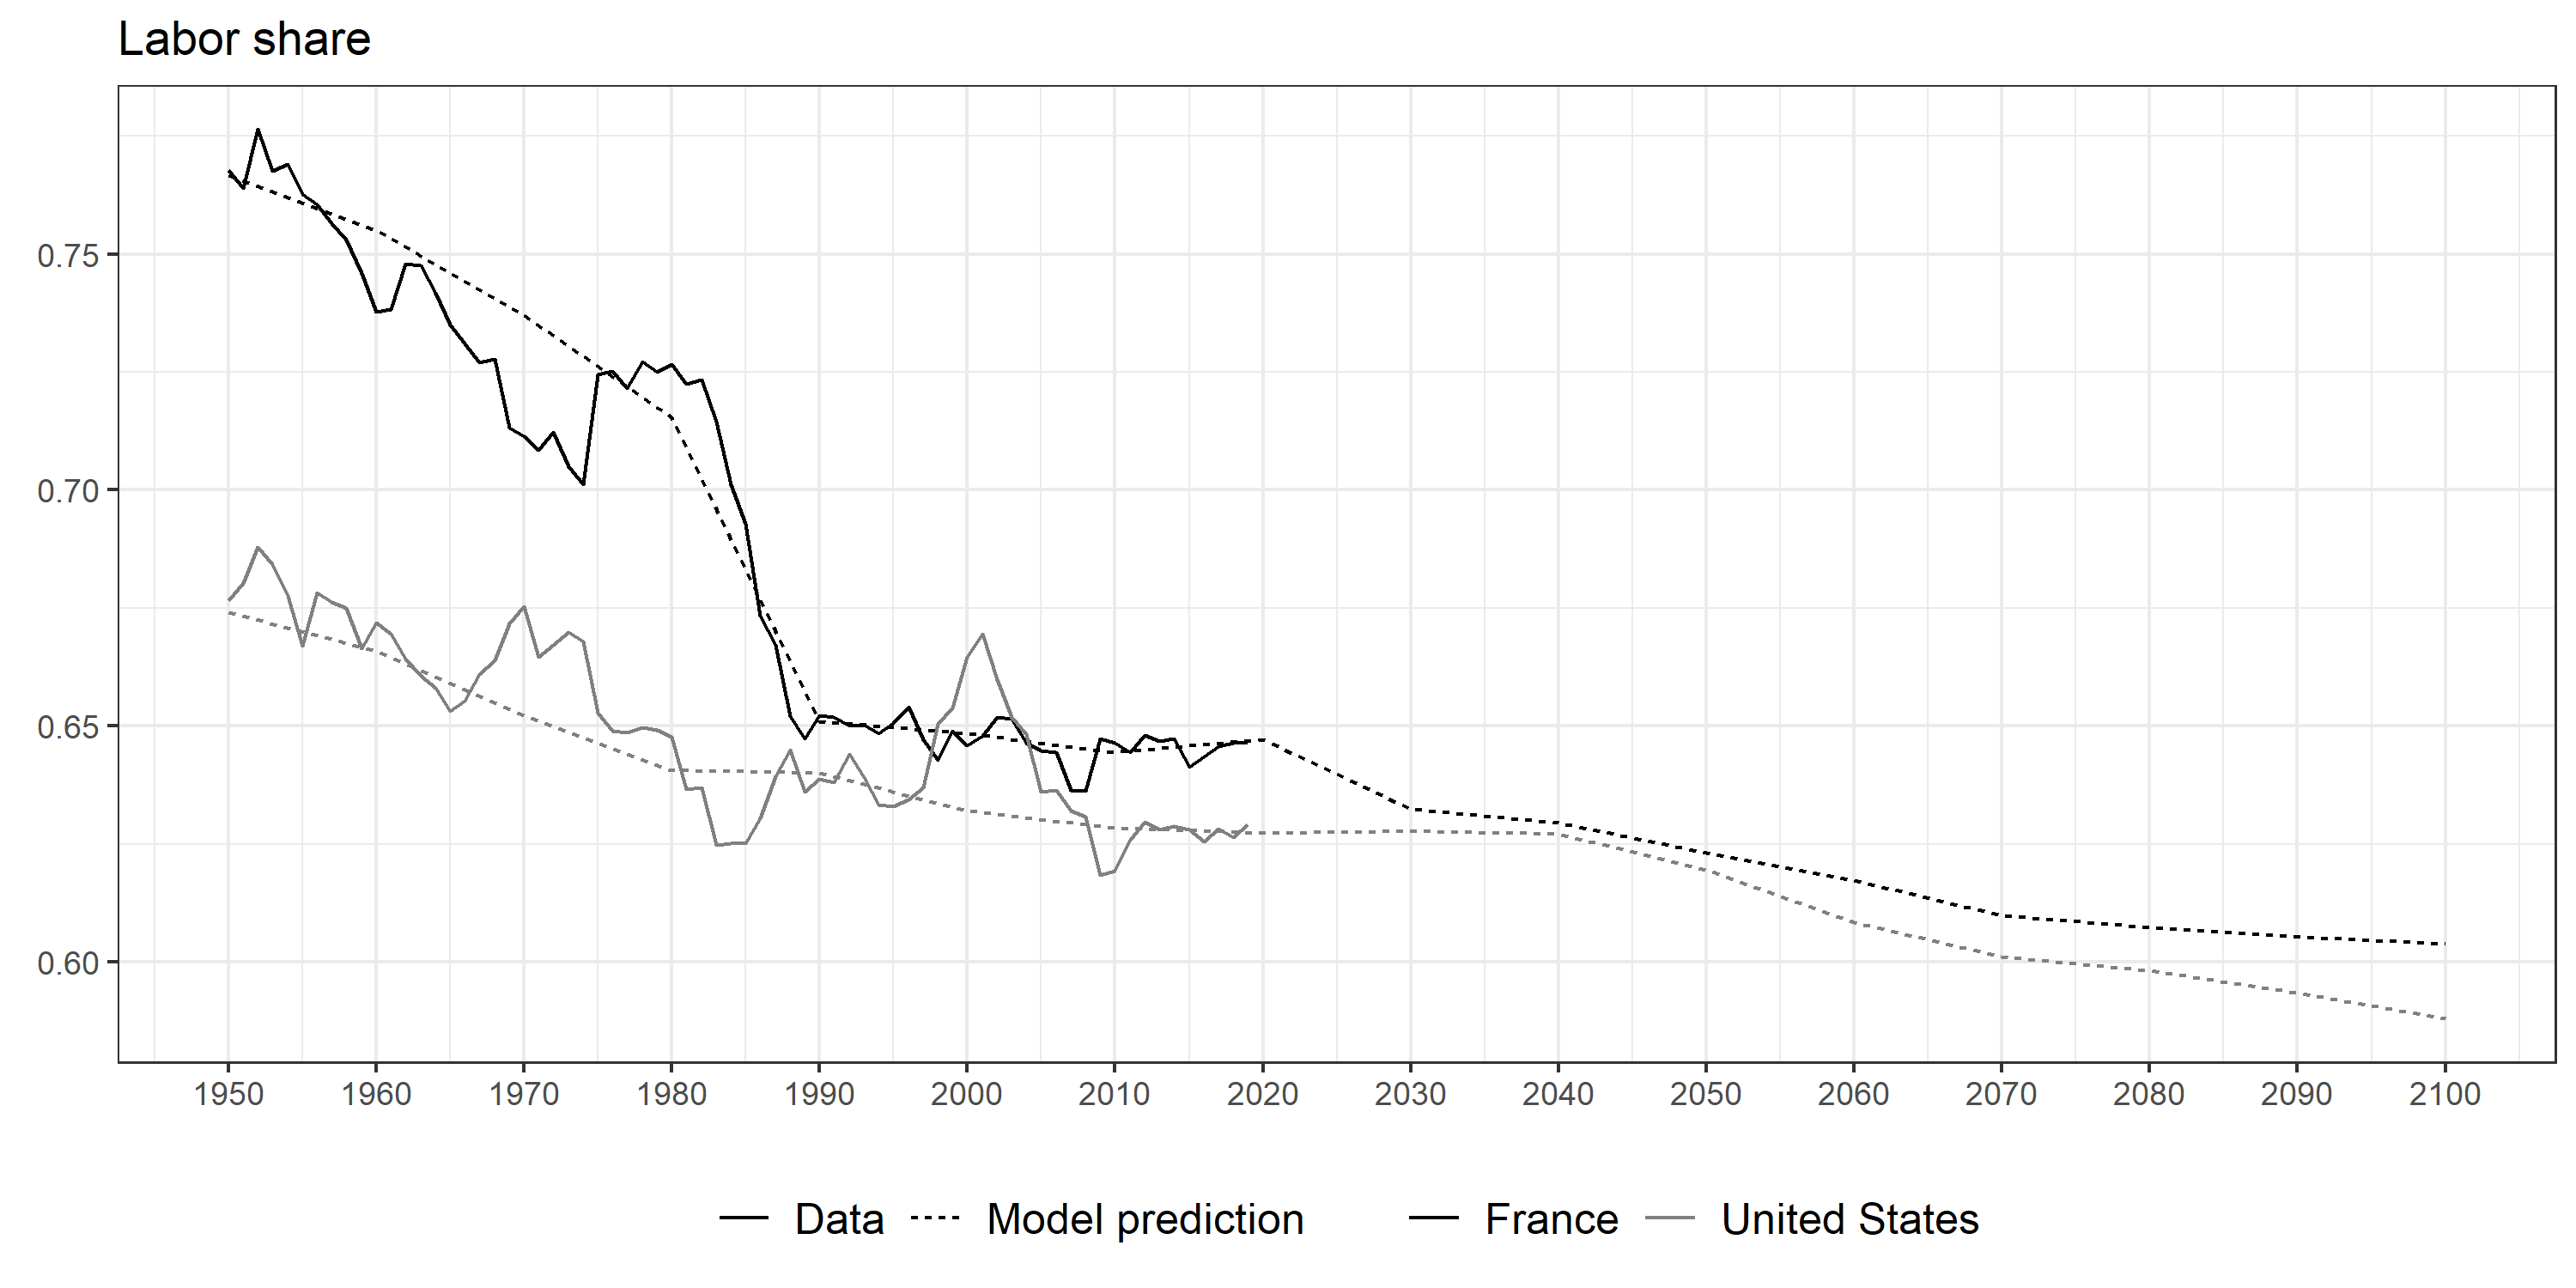
\includegraphics[width=1\linewidth]{chap1/graphic/quant-bench-ls.png}
	\vspace{-3em}
	\justify\singlespacing\footnotesize\textit{Notes:} The figure shows the labor share predictions of the model (dashed lines) and the labor share in the data (solid lines) from 1950 to 2100 for France and the US.
	Labor share data are from the \href{https://www.rug.nl/ggdc/productivity/pwt/}{Penn World Table 10.1} with self-employed income as labor compensation.
\end{figure}
The model reproduces the global trend in the data for both countries until 2020. For the US, the model underestimates the labor share around 2000. However, it captures the overall trend of the labor share over the period.
For France, model predictions are more accurate and reproduce the data since 1950. Looking at the model's predictions after 2020, the labor share should decline until the end of the century in both countries. I discuss the dynamics of variables---in the public policy equilibrium and in the labor market equilibrium---over the three periods: when the boomers are young (1970-2010), when they are retired (2010-2050), and afterward (2050-2100).

%% Other economic variables before 2010
\textbf{The young boomers (1970-2010).} 
Figure \ref{chap1-fig:quant-bench-dev7010-pub} displays the dynamics of public policy variables, expressed in percentage deviation from their 1970's value.
\begin{figure}[!tb]
	\centering
	\caption{Public policy dynamics over the 1970-2010 period} \label{chap1-fig:quant-bench-dev7010-pub}
	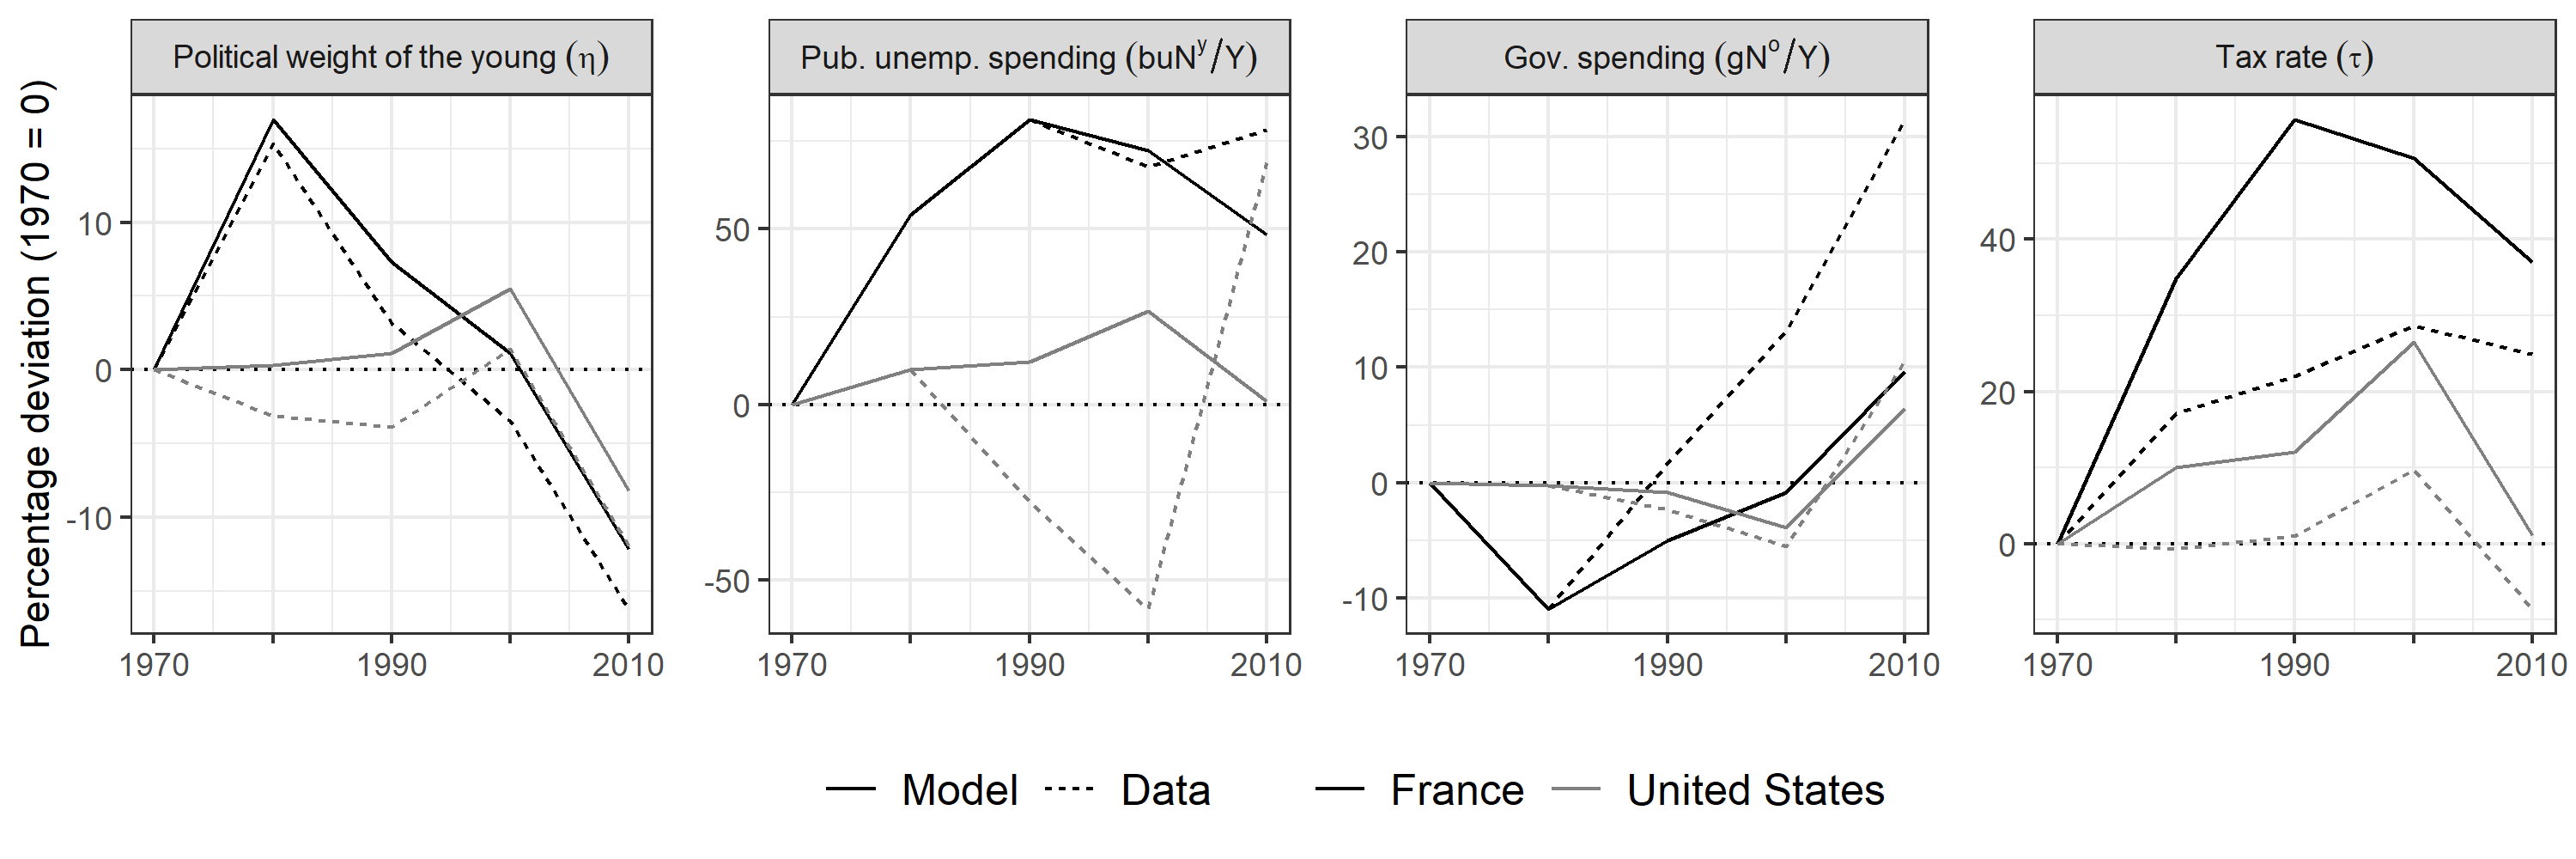
\includegraphics[width=1\linewidth]{chap1/graphic/quant-bench-dev7010-pub.png}
	\vspace{-3em}
	\justify\singlespacing\footnotesize\textit{Notes:} The figure shows the deviation of the variables from the public policy equilibrium from their 1970's value (in percentage) for France and the United States over the 1970-2010 period. Solid lines represent the dynamics obtained from the model simulation, dashed  lines represent the data, and the dotted line represents the 0-degree line.
\end{figure}
% Demographic context (n and p)
The rate of population growth $n_t$ slightly exceeds the increasing survival rate $p_t$ between 1970 and 2000. Thus, the old-age-dependency ratio $p_t/n_t$ remains roughly stable, although it declines slightly in France between 1980 and 1990 due to the massive entry of the boomers into the labor force. The old-age-dependency ratio starts to increase around 2000 due to a steady population growth combined with a sharply increasing survival rate, the boomers' generation starting to retire. As a result of this demographic context, the political weight of the young $\eta_t$ is above its 1970's level until 2000 in both countries as depicted in the first panel of the figure.

As the political weight of the young boomers rises, pro-youth policies are implemented due to the opportunistic behavior of political parties. These policies consist of more redistribution, i.e. a greater tax rate and more unemployment benefits, to prevent the income losses due to unemployment of the young boomers. Thus, the old-age specific government spending also decline, before increasing again as the boomer cohort starts to retire in 2010. Since the unemployment benefits act as an outside option for the workers, these public policy dynamics have consequences on the labor market.

Figure \ref{chap1-fig:quant-bench-dev7010-labor} displays the dynamics of labor market variables, expressed in percentage deviation from their 1970's value.
\begin{figure}[!tb]
	\centering
	\caption{Labor market dynamics over the 1970-2010 period} \label{chap1-fig:quant-bench-dev7010-labor}
	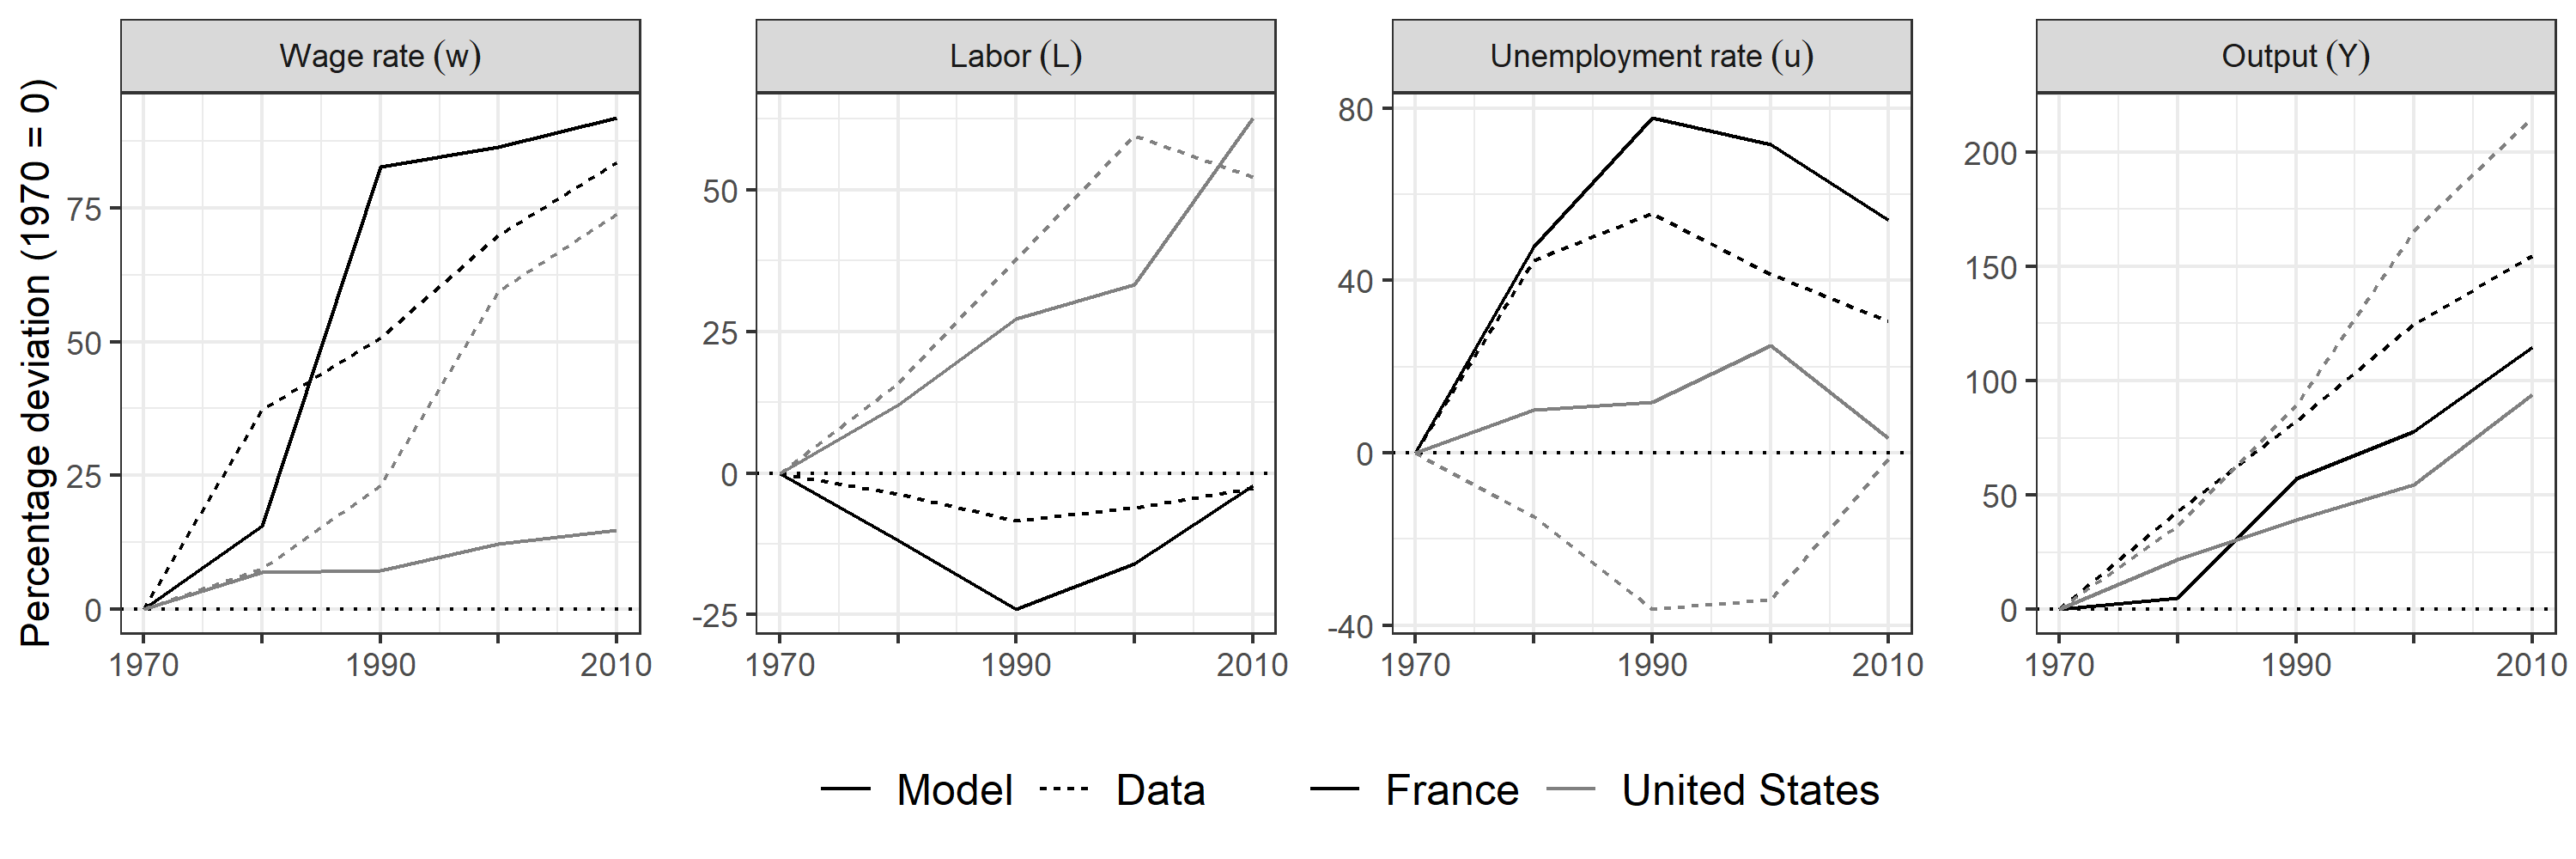
\includegraphics[width=1\linewidth]{chap1/graphic/quant-bench-dev7010-labor.png}
	\vspace{-3em}
	\justify\singlespacing\footnotesize\textit{Notes:} The figure shows the deviation of the variables from the labor market equilibrium from their 1970's value (in percentage) for France and the United States over the 1970-2010 period. Solid lines represent the dynamics obtained from the model simulation, dashed  lines represent the data, and the dotted line represents the 0-degree line.
\end{figure}
Workers can bargain greater wages as their outside option increases. Because the labor cost (i.e. the wage) increases for firms, they shift away from labor. This behavior is permitted by two features of the model. 
First, the monopsony position of the firm in the labor market enables the firm to hire and fire as much as wanted. 
Second, the capital-labor elasticity of substitution $\sigma$ is greater than one, thus, both input factors are gross substitutes and the firm is all the more able to substitute labor with capital for a given output level. This behavior leads to a decline of the number of workers $L_t$ in France and a moderate increase in the US, as highlighted in the second panel. The diverging patterns between the two countries are due to the substitution effect being stronger in France than in the US. The higher elasticity of substitution in France combined with faster growth of the capital stock $K_t$ pushes French firms to substitute relatively more labor with capital. Thus, the number of workers becomes lower than its 1970's level in France, whereas the US manage to slightly increase their labor factor because the increase in wages is not as strong as in France.

This fall in employment raises unemployment in France, the effect being enhanced by the labor force growth due to the number of young boomers. For the US, the moderate increase in labor does not manage to offset population growth. Therefore, the unemployment rate also raises as depicted in the third panel. Since both factors are gross substitutes, output $Y_t$ and output-per-worker grow along with capital-per-worker. The increase in output per worker exceeds the one of the wages, and as a result, the labor share declines.

The mechanisms until 2010 can be summarized as follows. The young boomers change labor market institutions in their favor due to their relatively high political weight. This raises the outside option of workers and hence their bargaining power, enabling them to bargain greater wages. Labor becoming costly, firms decide to shift away toward capital. This shift-away from labor engenders an increase in output-per-worker that exceeds the wage gain; thus, the labor share declines. 

\textbf{The retired boomers (2010-2050) and afterward (2050-2100).} Dynamics of the same set of variables also help to highlight the mechanisms of the model's predictions for the labor share after 2010.
Figure \ref{chap1-fig:quant-bench-dev1000-pub} displays the dynamics of public policy variables, expressed in percentage deviation from their 2010's value.
\begin{figure}[!tb]
	\centering
	\caption{Public policy dynamics over the 2010-2100 period} \label{chap1-fig:quant-bench-dev1000-pub}
	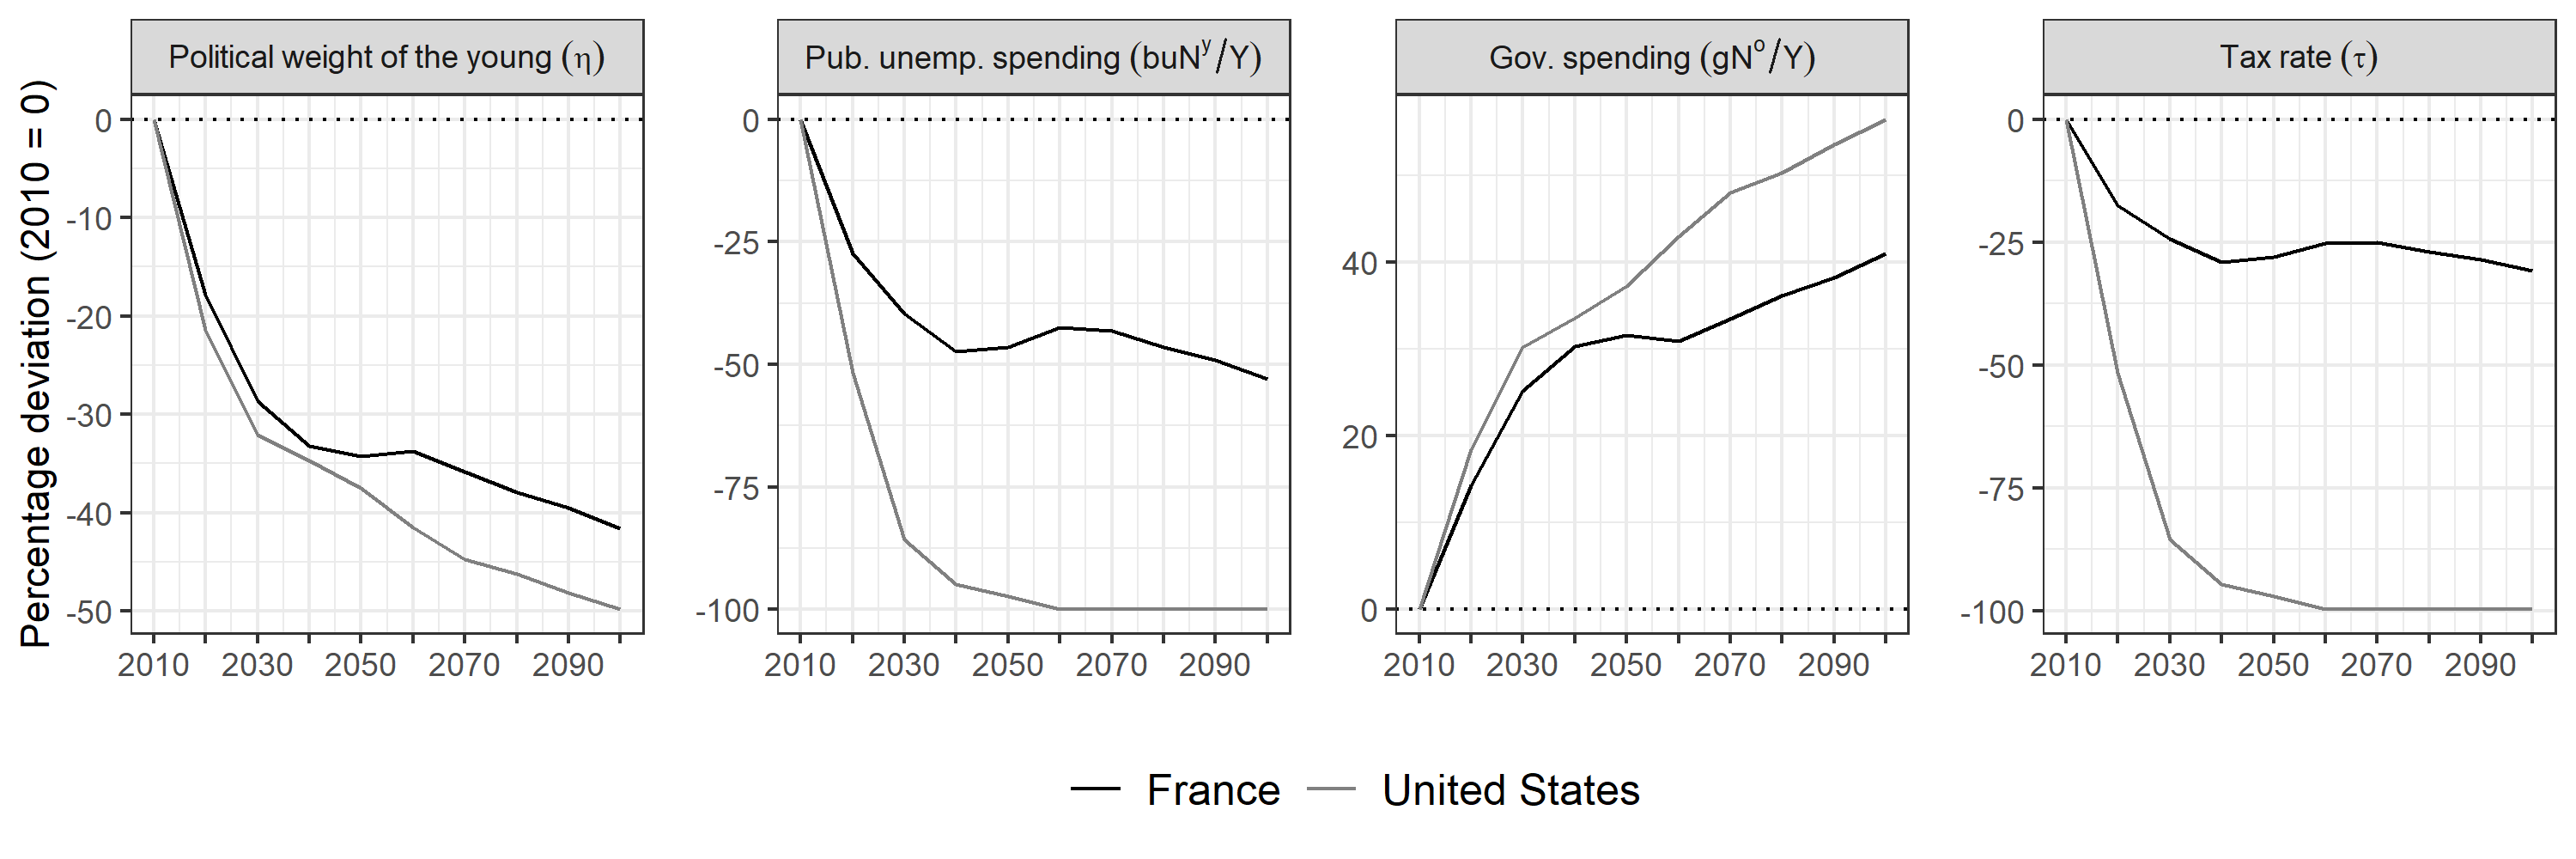
\includegraphics[width=1\linewidth]{chap1/graphic/quant-bench-dev1000-pub.png}
	\vspace{-3em}
	\justify\singlespacing\footnotesize\textit{Notes:} The figure shows the deviation of the variables from the public policy equilibrium from their 2010's value (in percentage) for France and the United States over the 2010-2100 period. Solid lines represent the dynamics obtained from the model simulation and the dotted line represents the 0-degree line.
\end{figure}
The demographic context over this period is the following: the rate of population growth $n_t$ declines sharply between 2010 and 2050 before stabilizing thereafter. Meanwhile, the survival rate $p_t$ grows by around 4\% per decade. Thus, the old-age-dependency ratio sharply increases from 2010 to 2050. Once the rate of population growth becomes stable, the old-age-dependency ratio still grows but at a lower rate. As a result, the political weight of the young, $\eta_t$, never returns to its 2010 level and strongly declines until 2050 for both countries as shown in the first panel.

As the political weight of the young declines, the reverse of the mechanism that led to the decline of the labor share when the boomers were young is expected. Opportunistic political parties favor the retired boomers and implement pro-elderly public policies, i.e. a lower tax rate and more old-age specific government spending. Thus, unemployment benefits decline and so does the outside option of workers. These changes in public policy have consequences on the labor market.

Figure \ref{chap1-fig:quant-bench-dev1000-labor} displays the dynamics of public policy variables, expressed in percentage deviation from their 2010's value.
\begin{figure}[!tb]
	\centering
	\caption{Labor market dynamics over the 2010-2100 period} \label{chap1-fig:quant-bench-dev1000-labor}
	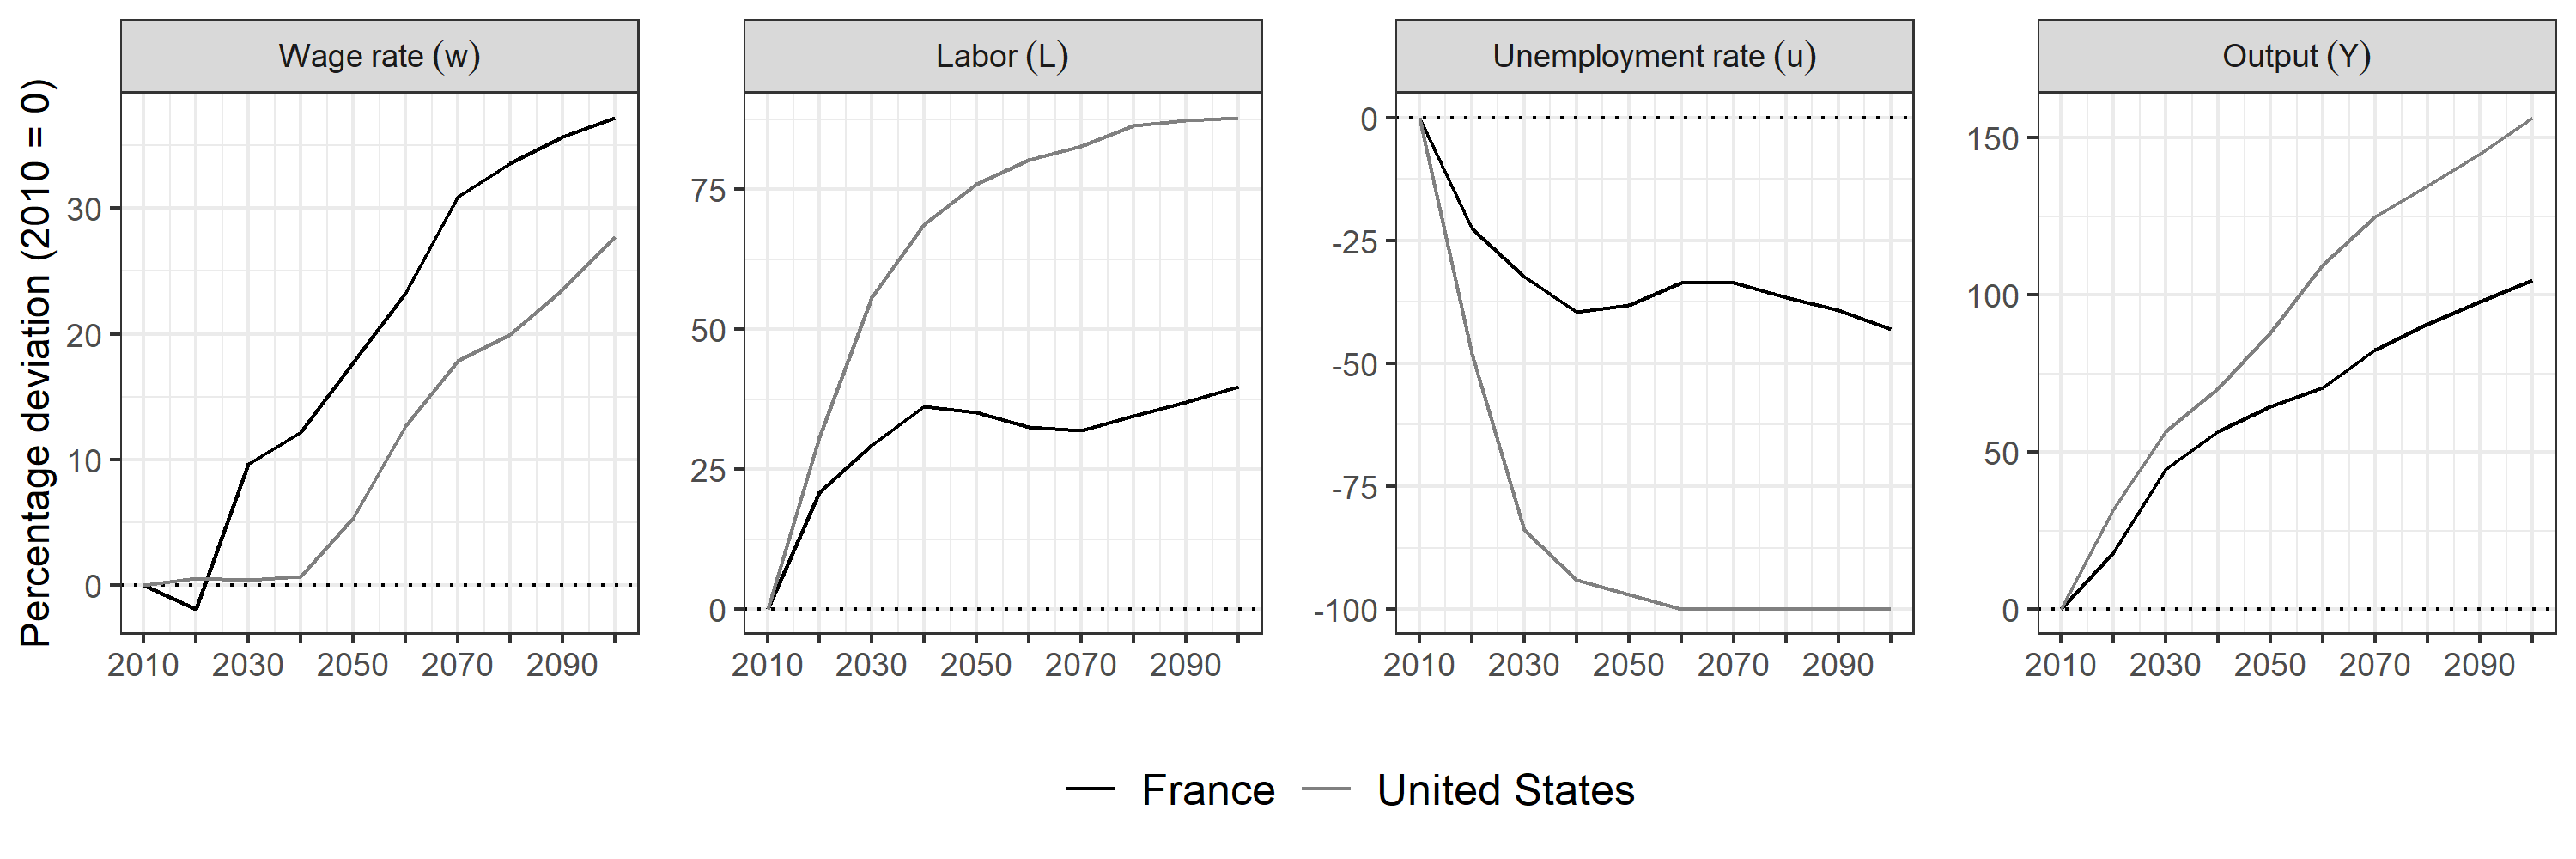
\includegraphics[width=1\linewidth]{chap1/graphic/quant-bench-dev1000-labor.png}
	\vspace{-3em}
	\justify\singlespacing\footnotesize\textit{Notes:} The figure shows the deviation of the variables from the labor market equilibrium from their 2010's value (in percentage) for France and the United States over the 2010-2100 period. Solid lines represent the dynamics obtained from the model simulation and the dotted line represents the 0-degree line.
\end{figure}
As a result, they concede a wage stagnation inciting firms to hire more, as depicted in the second panel. The unemployment rate drops due to higher employment combined with the decline of the rate of population growth, as shown in the third panel.

Nonetheless, the labor share never recovers its 2010's level. The dynamics of the labor share are governed by two factors: an increase in employment and a higher capital stock arising from the savings of the boomers when they were young. These savings were fostered by the size of the boomer generation; the rising expected life expectancy; and the high level of their wages. While higher employment tends to increase the labor share, the larger stock of capital tends to reduce it, keeping the labor share roughly stable in both countries when the boomers are retired.

Once the boomers pass away, after 2050, the decline in the political power of the young slows down in both countries. This slowdown allows workers to bargain greater wages. French firms substitute labor with capital to thwart workers' appropriation of the rents, leading to a decline of the labor factor and so a rise in unemployment. On the other side of the Atlantic, firms in the US manage to hire until full-employment due to the sharp increase in capital and the stagnation of the labor supply. However, the wage gains remain lower than the rise in output-per-worker in both countries. Therefore, both labor shares decline to reach 60.4\% in France and 58.8\% in the US by 2100, while their respective levels were about 64.5\% and 62.8\% in 2010.

The mechanisms after 2010 can be summarized as follows. The boomers retire and change the public policy in their favor, reducing taxes and unemployment benefits which raises employment. The positive effect of employment on the labor share is dampened by capital accumulation due to the extensive savings of the boomers when they were young. Consequently, the labor share slightly increases in France and stabilizes in the US, before declining again by the end of the century due to the aging of the population.

\subsection{Factor-accumulation and policy-mechanism effects} \label{chap1-counterfactual}

% Mechanisms so far
So far I have highlighted the different mechanisms through which the age structure of the population affects economic variables and therefore the labor share. Demographic changes are due to changes in two exogenous variables: the population growth rate $n_t$ and the survival rate $p_t$. 
Their dynamics may affect the labor share through two channels: the \textit{direct factor-accumulation} effect and the \textit{indirect policy-mechanism} effect.

% Quantify
To quantify the respective role of each effect, I make counterfactual simulations. In these simulations, I neutralize a channel of demographic changes by setting it to its level in 1970, i.e. the decade before the massive entry of the boomers on the labor market.
% Initial values
Table \ref{chap1-tab:quant-demo70} summarizes the demographic variables in 1970.
\begin{table}[!tb]
    \centering
    \begin{threeparttable}
        \caption{Demographic variables in 1970} \label{chap1-tab:quant-demo70}
        
\begin{tabular}{llrr}
\toprule
\textbf{} & \textbf{Variable} & \textbf{France} & \textbf{United States}\\
\midrule
$n_{1970}$ & Population growth rate & 1.134 & 1.597\\
$p_{1970}$ & Survival rate & 0.417 & 0.476\\
$p_{1990}$ & Expected survival rate & 0.583 & 0.561\\
$\frac{p_{1970}}{n_{1970}}$ & Old-age dependency ratio & 0.368 & 0.298\\
$\eta_{1970}$ & Young political weight of the young & 4.169 & 2.869\\
\bottomrule
\end{tabular}

        \begin{tablenotes}[flushleft]
            \footnotesize{\item \textit{Notes}: The table reports the demographic variables in 1970 for France and the United States. 
            % Data are from the benchmark simulation of the model.
            }
        \end{tablenotes}
    \end{threeparttable}
\end{table}
Then, I compare counterfactual simulations to the benchmark obtained in section \ref{chap1-model_pred}, thus, I quantify to which extent each channels affect the labor share. For more details on the methodology to construct the counterfactual simulations, see appendix \ref{chap1-countermetho}.

% Direct vs indirect
To neutralize the factor accumulation effect, I suppose that all demographic parameters remain at their 1970's level, i.e. $n^\prime_t = n_{1970}$ and $p^\prime_t = p^\prime_{t+1} = p_{1970}$, which affects population dynamics and the saving rate. In this simulation, only the political weight of the young remains identical to the benchmark simulation, i.e. $\eta_t^\prime = \eta_t$. Conversely, I neutralize the policy mechanism effect by setting the political weight of the young to its level in 1970, i.e. $\eta^\prime_t = \eta_{1970}$, while all demographic parameters remain at their benchmark values. Lastly, I make a counterfactual simulation to neutralize both channels in which $n^\prime_t = n_{1970}$, $p^\prime_t = p^\prime_{t+1} = p_{1970}$ and $\eta_t^\prime = \eta_{1970}$. This latter simulation is the baseline counterfactual simulation.

% Figure for direct vs indirect
Figure \ref{chap1-fig:quant-decomp-channel} presents the sizes of the factor accumulation effect and the policy mechanism effect, derived from the counterfactual simulations, in percentage points.
\begin{figure}[!tb]
	\centering
	\caption{Decomposition of the channels of demographic changes} \label{chap1-fig:quant-decomp-channel}
	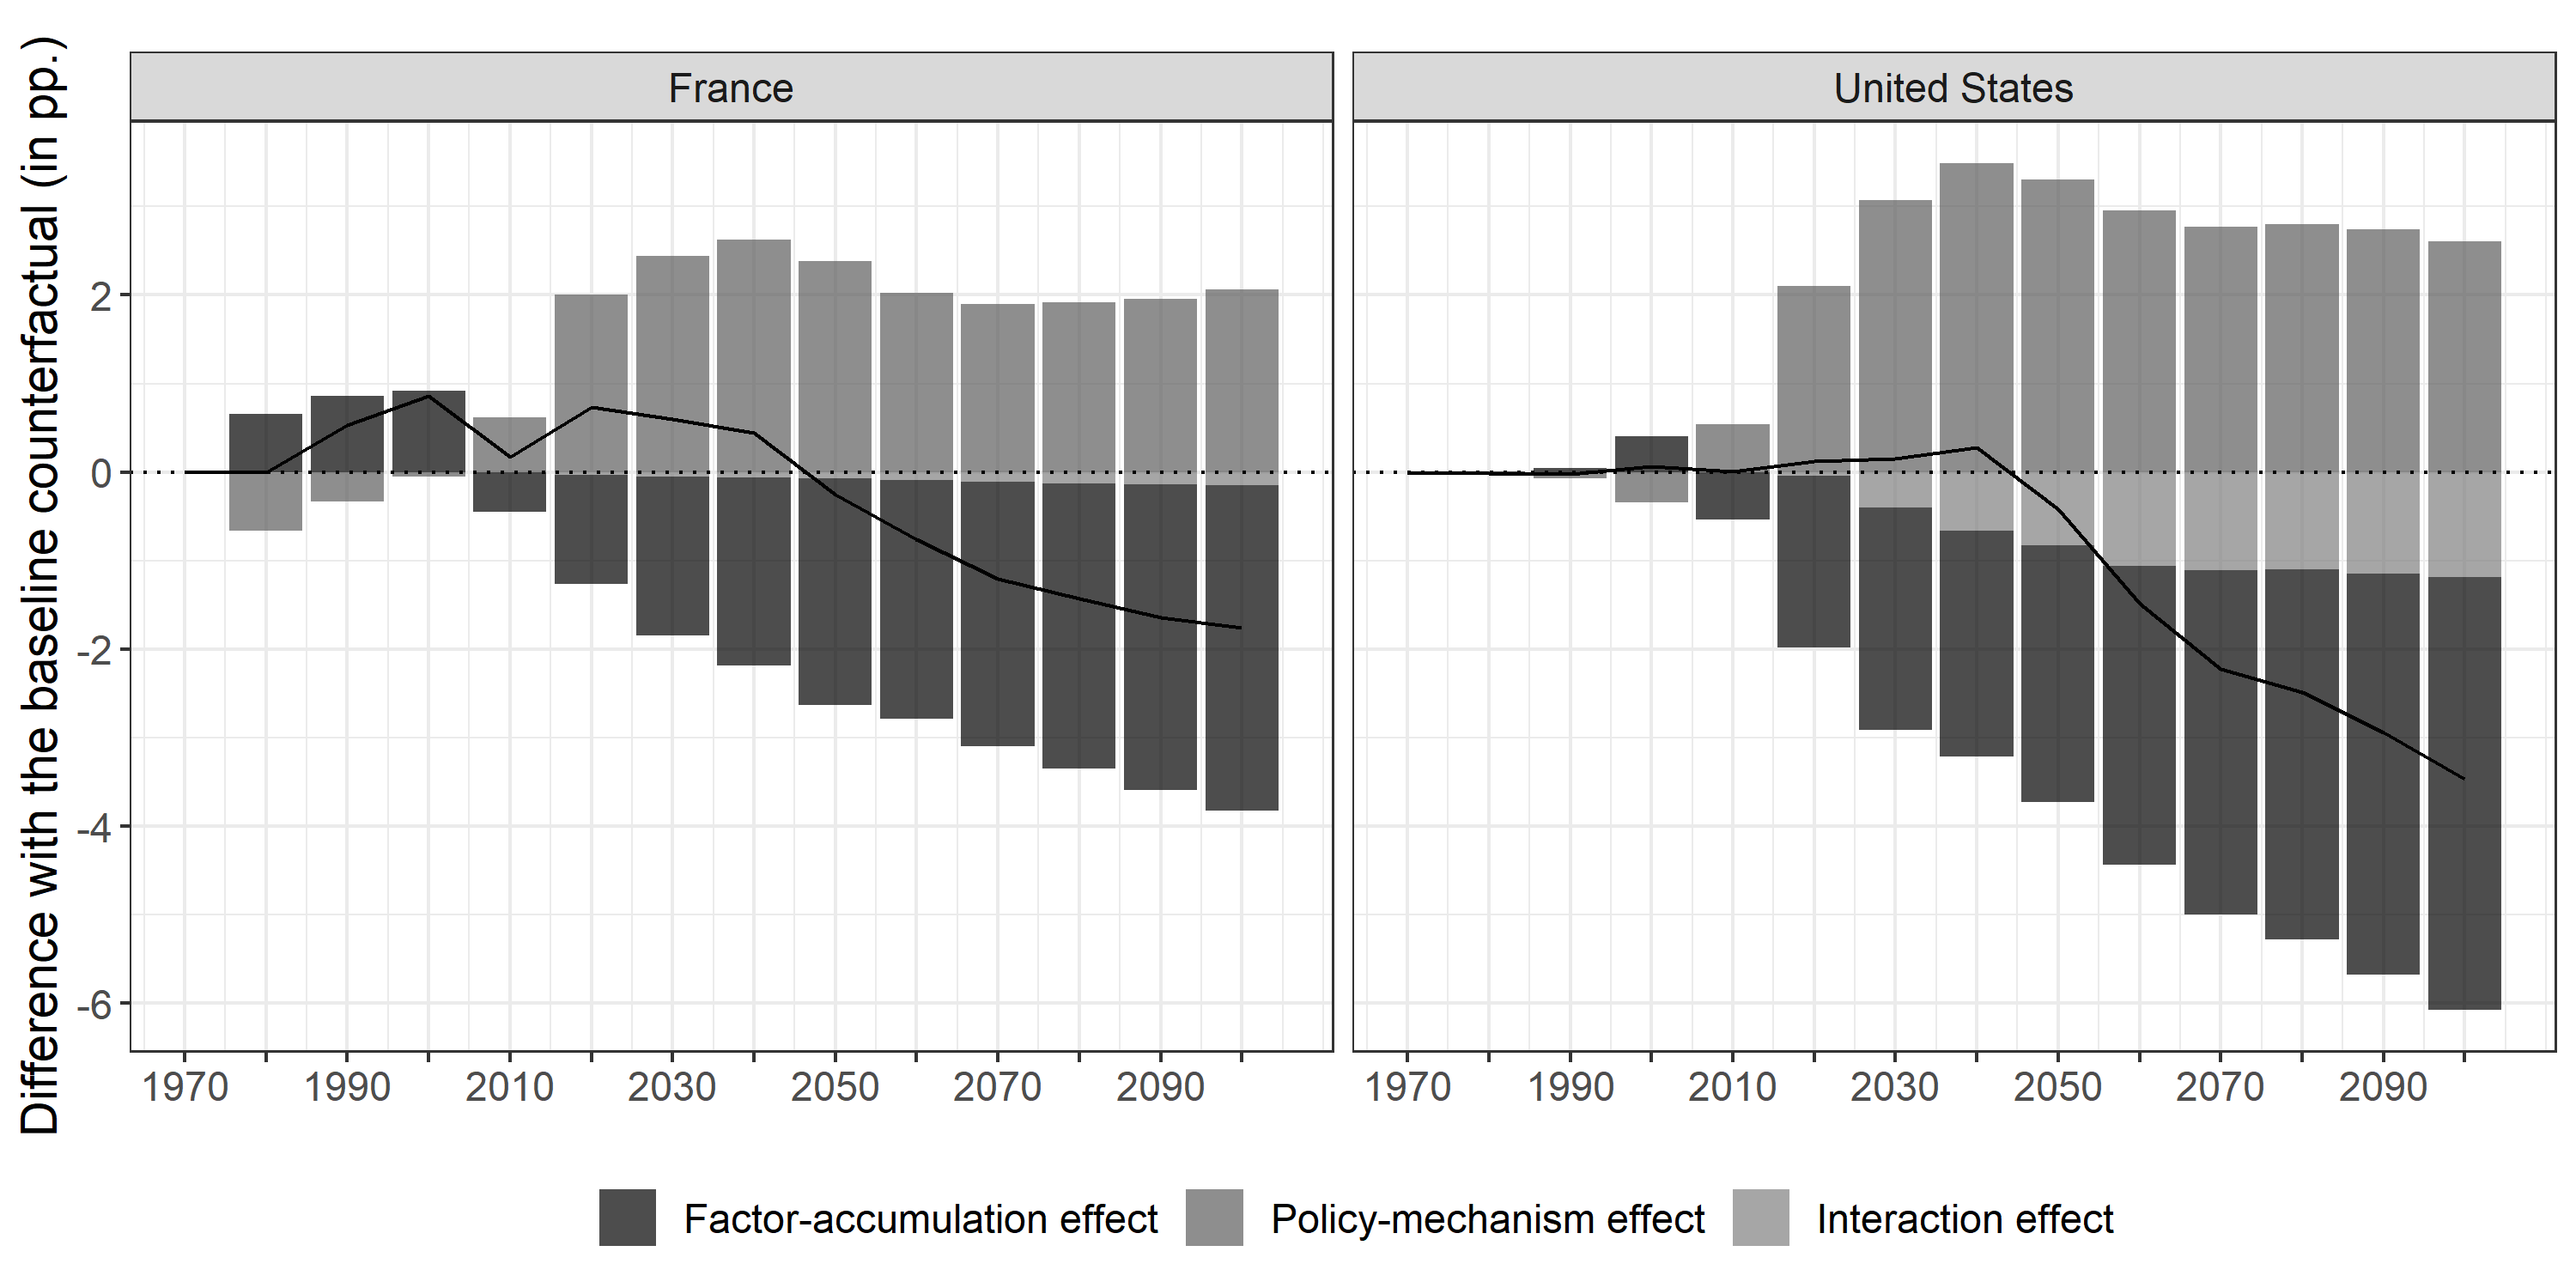
\includegraphics[width=1\linewidth]{chap1/graphic/quant-decomp-channel.png}
	\vspace{-3em}
	\justify\singlespacing\footnotesize\textit{Notes:} The figure shows the decomposition of the channels of demographic changes on the labor share. Effects are expressed in percentage point difference with the baseline counterfactual simulation. The baseline counterfactual corresponds to the simulation where all the demographic variables and the young political weight remain at their initial levels. The factor-accumulation effect accounts for the effect of demographic changes through the factor-accumulation channel on the labor share, while the policy-mechanism effect accounts for the effect of demographic changes through the policy-mechanism channel. Both effects are obtained by taking the difference between the benchmark labor share and the labor share from the simulation in which the channel is canceled. The interaction effect is defined as the part which is not exclusively explained by both effects independently. The solid line represents the net effect corresponding to the sum of the three effects, that is also the difference between the labor shares from the benchmark and the baseline counterfactual simulation.
\end{figure}
% Direct mostly positive % Increasing Ny => low wages => increases L
The factor-accumulation effect is mostly positive when the boomers are young, because the increasing labor supply is in favor of firms within the bargaining, keeping wages low which fosters employment. 
% In addition, the saving rate remains low and so does the capital stock.
Meanwhile, the policy-mechanism effect harms the labor share, owing to the rise of the young boomers' political weight which increases their unemployment benefits, hence wages, and therefore incites firms to shift away from labor toward capital.

% AFTER 2010: boomers retire, both effects are reversed
Once the boomers start to retire in 2010, both effects are reversed. The policy-mechanism effect becomes positive because old boomers foster pro-elderly public policy. This change in the policy is done at the cost of labor market insurance. Thus, workers are not able to bargain greater wages which fosters labor demand. Nonetheless, the factor-accumulation effect is negative because of the large amount of available capital stock due to the savings of the boomers when they were young. As a result, the factor-accumulation effect offsets the positive impact on the labor share of the reversal policy-mechanism effect.

% % \textbf{Summary of the effects.} 
% Figure \ref{chap1-fig:quant-decomp-sum} summarizes the relative share of the effects of demographic changes on the labor share by period and country.
% \begin{figure}[!tb]
% 	\centering
% 	\caption{Relative share of the effects of demographic changes on the labor share} \label{chap1-fig:quant-decomp-sum}
% 	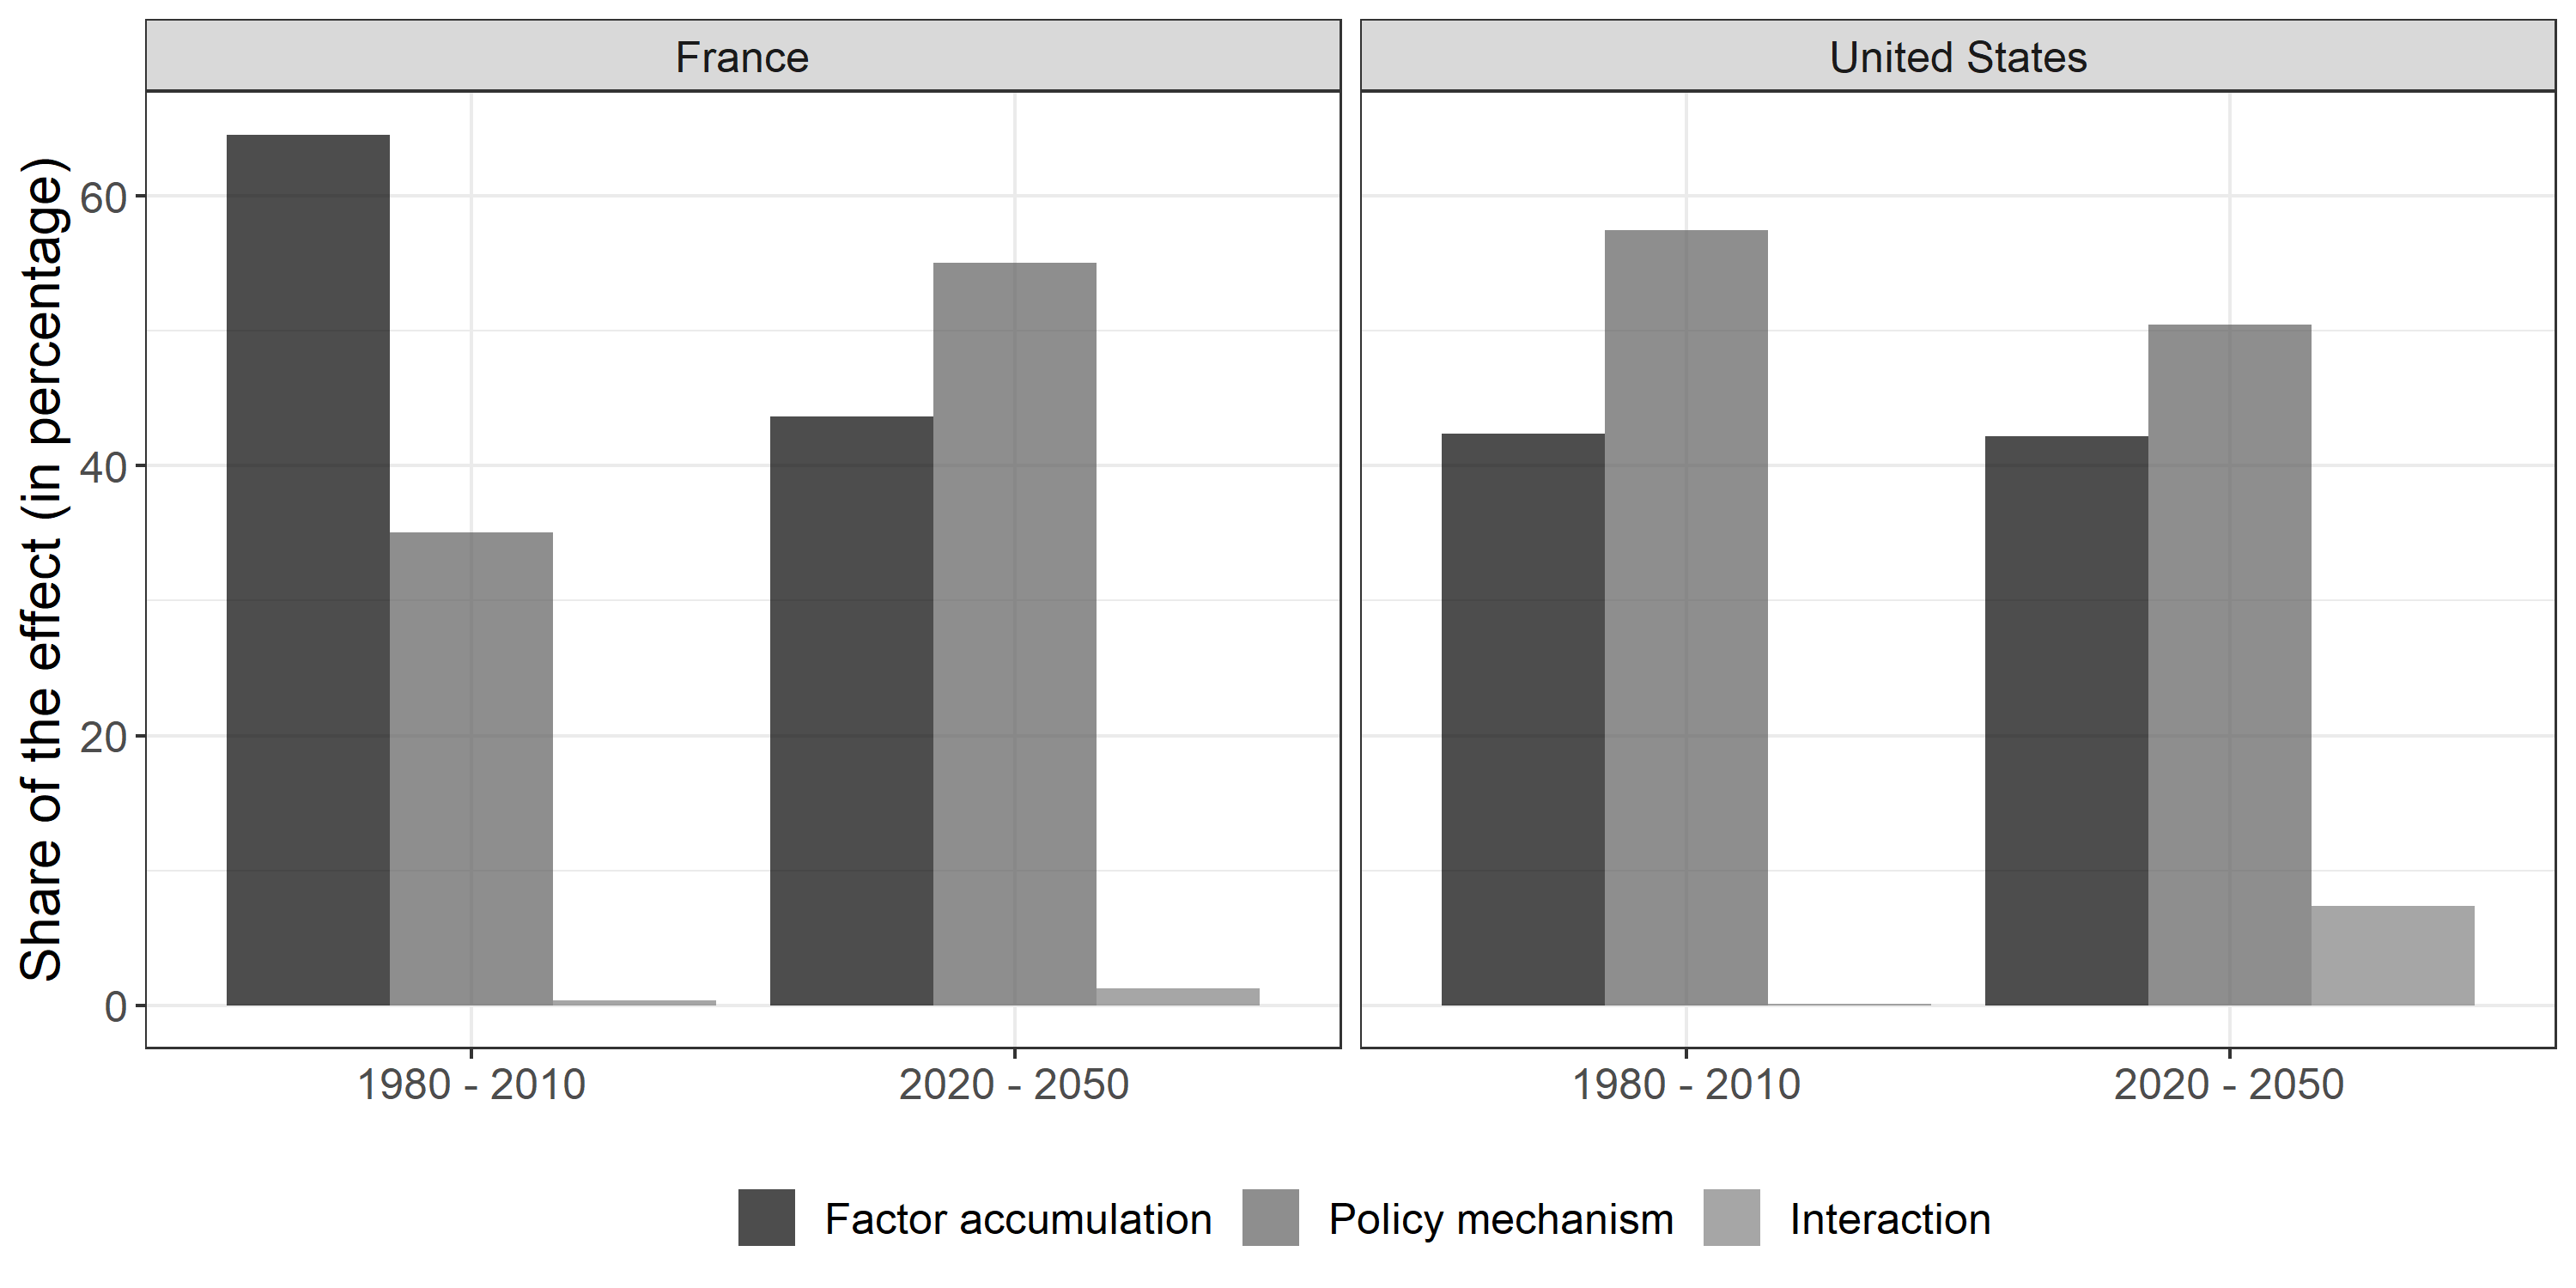
\includegraphics[width=1\linewidth]{chap1/graphic/quant-decomp-sum.png}
% 	\vspace{-3em}
% 	\justify\singlespacing\footnotesize\textit{Notes:} The figure shows the average percentage relative share of the channels of demographic changes on the labor share over the two periods of the boomers generation (young and old), for France and the United States. Data are from the counterfactual simulations of the model and summarize the results from figure \ref{chap1-fig:quant-decomp-channel}.
% \end{figure}
% Changes in the population growth rate and survival rate affect the labor share through two channels: the factor-accumulation effect and the policy-mechanism effect. When the boomers are young, the factor-accumulation effect dominates in France while the policy-mechanism effect prevails in the US. On average, the share explained by the policy-mechanism effect is about 35\% in France and 57.5\% in the US. Thereafter, between 2020 and 2050, the share of this latter effect rises by 20.8 pp. in France becoming the main channel, while it slightly decreases by 7 pp. in the US. These results suggest that the policy-mechanism effect accounts for more than half of the consequences of demographic dynamics on the labor share.

% Compare with SV2013
\citet{Schmidt2013Demographic} consider only the factor accumulation mechanism and show that this mechanism disappears in a small open economy because capital-per-worker and the wage rate are independent of domestic savings, so that labor share dynamics only reflect changes in net foreign assets.
% My approach
The major advantage of my approach is that the policy mechanism holds in a small open economy.
%
With capital mobility, \citet{Pica2010Capital} argues that competition to attract capital between countries leads to reduced labor market regulation and a lower labor share.
%
Nonetheless, he uses a Cobb-Douglas production function which cancels out the shift away from labor toward capital of firms that is allowed by the CES production function that I employ.
%
In terms of consequences for the labor share, the effect of capital markets integration that occurs through labor market deregulation in an open economy is equivalent to the response of the firms that substitute labor with capital to thwart workers' appropriation of the rents in a closed economy.

\subsection{Age-related conflict: who are the winners ?} \label{chap1-winners}

% So far
The results show that the labor share declines due to the size of the boomers' cohort in France and the US. First, when they are young they shape labor market institutions in their favor, raising wages but inciting firms to shift away from labor toward capital. Second, when they are old they have substantially increased the available capital in the economy through their savings, pushing firms to substitute even more. Although it may seem obvious that the boomers are the winners of the age-related conflict when they are old, the results raise the question of whether they were the losers when they were young because the labor share declined considerably over this period.

Although much emphasis is given to it in the policy debate, the labor share is a gross indicator of the income distribution that does not take into account redistribution. The net income ratio between young and old is more appropriate to determine the winners of the age-related conflict.\footnote{I do not consider the difference in lifetime utility between generations to assess who are the winners. The shape of the utility function does depend on the date at which a generation appears because the effective discount factor $\alpha p_{t+1}$ depends on life expectancy which varies across generations. Since two generations do not have the same baseline, then utility comparisons do not make much sense.}
Let $T$ be the per-capita redistribution from old to young that is the product between the old-age dependency ratio, i.e. $p_t/n_t$, and the difference between the after-tax and before-tax young-to-old income ratios, i.e. $Y_t^y/Y_t^o - \Theta_t$. Using equation \eqref{chap1-eq:after-tax-income-ratio},
\begin{equation*}
    T_t \equiv \frac{p_t}{n_t}\left(\frac{Y_t^y}{Y_t^o} - \Theta_t\right) =  \frac{p_t}{n_t}\left(\eta_t - \Theta_t\right).
\end{equation*}
Therefore, changes in per-capita redistribution reflect changes in the old-age dependency ratio, i.e. $p_t/n_t$, and in the aggregate redistribution, i.e. $\eta_t - \Theta_t$.

Figure \ref{chap1-fig:discuss-ratiopc} presents the per-capita redistribution from old to young in percentage deviation from its value in 1970.
\begin{figure}[!tb]
	\centering
	\caption{Per-capita redistribution dynamics} \label{chap1-fig:discuss-ratiopc}
	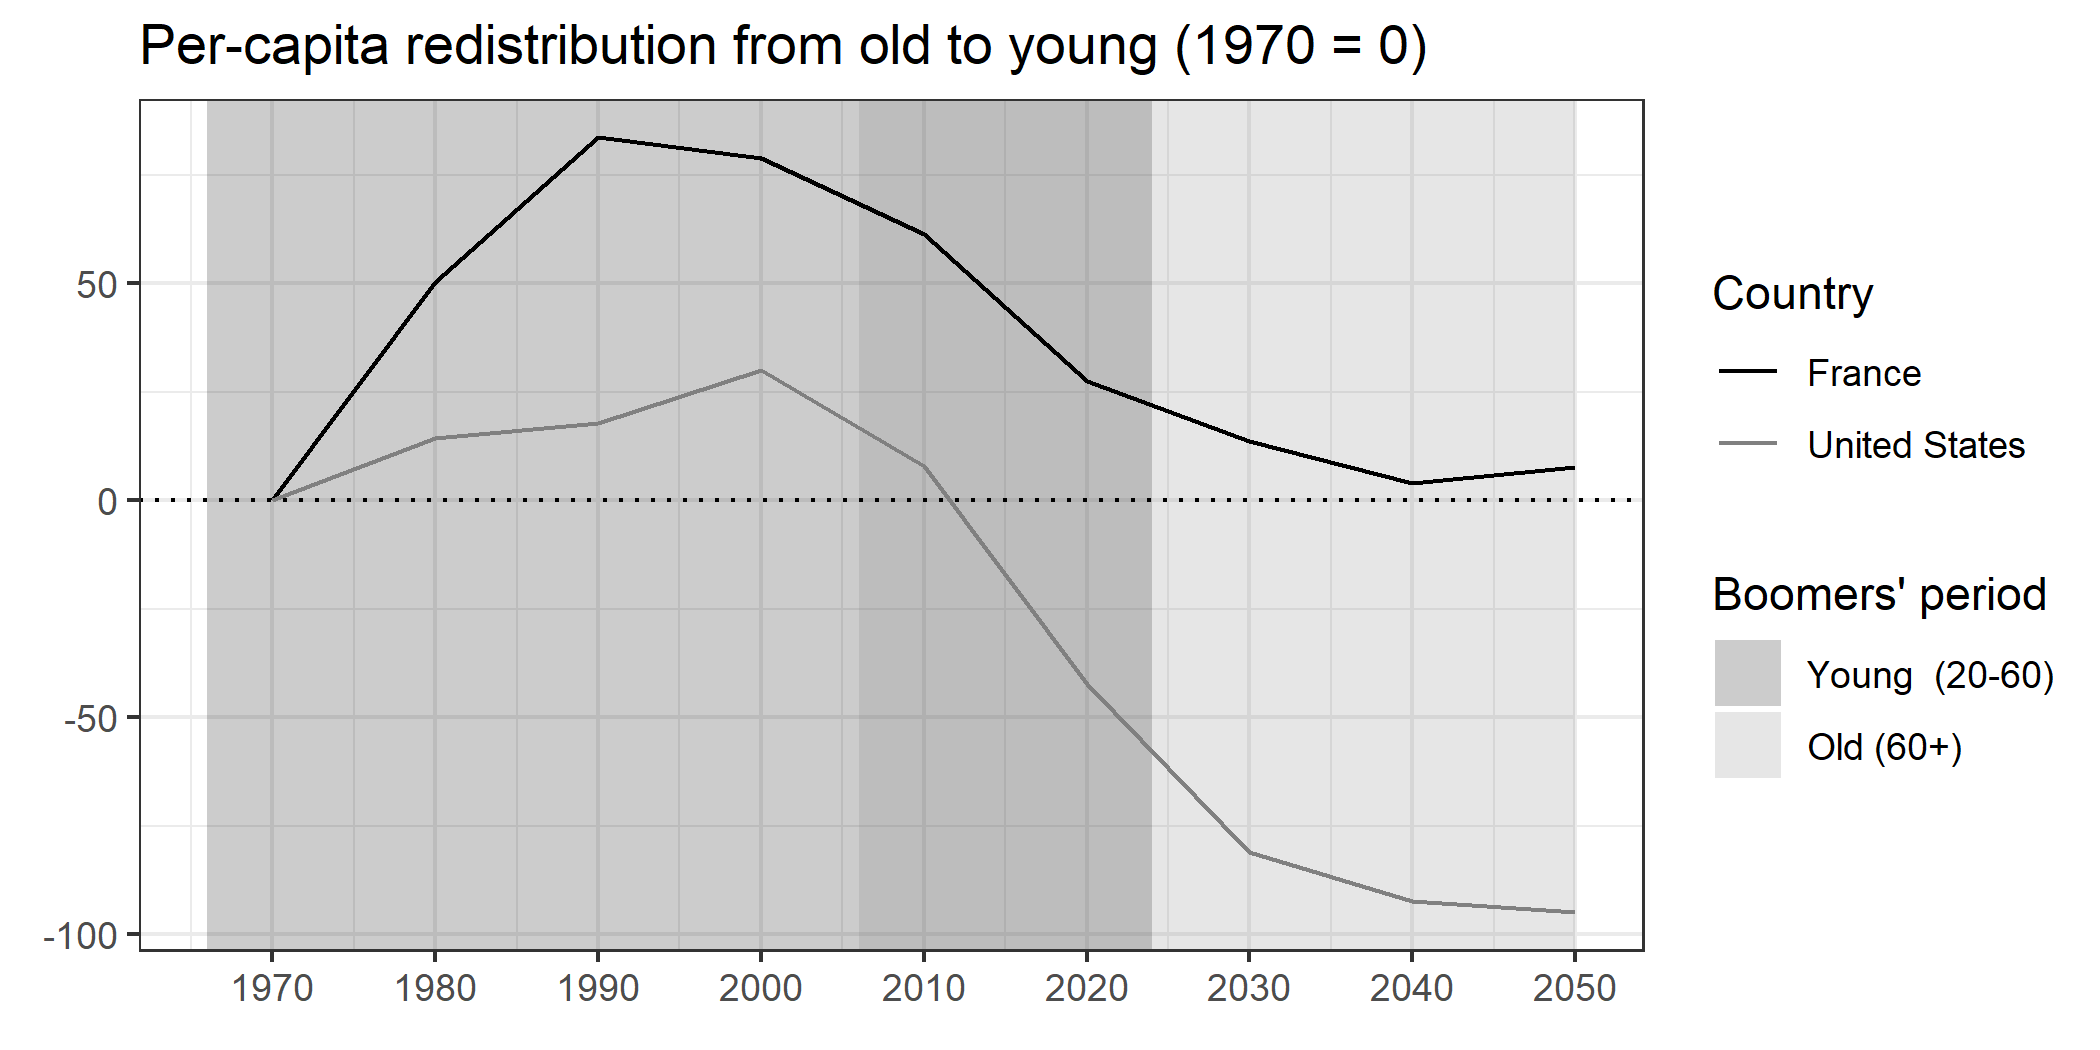
\includegraphics[width=1\linewidth]{chap1/graphic/discuss-ratiopc.png}
	\vspace{-3em}
	\justify\singlespacing\footnotesize\textit{Notes:} The figure shows the per-capita redistribution from old to young for France and the United States in percentage deviation since 1970. The black and grey lines represent, respectively, the France and the United States. The dotted line represents the 0-degree line. Rectangles define the periods when the boomers are young and old. Data are from the benchmark simulation of the model.
\end{figure}
When the boomers are young and enter the labor market (in 1970), they earn labor income until they start to retire in 2010. Over this period, the labor share declines and the per-capita redistribution from old to young increases in both countries. The young boomers are the winners of the age-related conflict over this period because they manage to recover their labor income losses by increasing redistribution due to their political weight. Once they retire and earn capital income, the labor share is rather stable, although the per-capita redistribution sharply declines. As a result, the boomers are also the winners of the age-related conflict when they are old because the level of redistribution from old to young declines. In the case of the US, the redistribution from old to young tends toward zero as the US economy is in full employment, hence, there is little need for unemployment benefits.\footnote{Note that the only source of heterogeneity is age, thus, there may be winners and losers within each cohort in presence of additional dimensions of heterogeneity, e.g. human capital.}